%!TEX root = ../template.tex
%%%%%%%%%%%%%%%%%%%%%%%%%%%%%%%%%%%%%%%%%%%%%%%%%%%%%%%%%%%%%%%%%%%%
%% chapter2.tex
%% NOVA thesis document file
%%
%% Chapter with the template manual
%%%%%%%%%%%%%%%%%%%%%%%%%%%%%%%%%%%%%%%%%%%%%%%%%%%%%%%%%%%%%%%%%%%%
\chapter{Related Work}
\label{cha:related_work}

This chapter presents and briefly discusses the related work and the study performed beforehand in order to guide and give some context to the reader. It will present work that was used as the basis of this thesis, existent technologies and their relation with this project, and some comparisons between those exiting technologies, the problem addressed in this thesis and the solutions proposed to solve, or better address, those very same problems.

First, in section 2.1 we explain and discuss for the first time the definition of a Key-Value Store. We  present some use cases, current technology available, their differences and most importantly their security models and concerns.

Having discussed the software, section 2.2 will then address the environment on where the previously talked software will run, most specifically the hardware. It explains and present the different ways to secure and authenticate the hardware, prevent hardware-based attacks and discuss some of the current products available and how they will be used across this thesis.

Section 2.3 will then make the bridge between software and hardware. It explains how Key-Value stores are currently being run on secure environments. 
This chapter will be focused on the Intel SGX secure model and explain the advantages and disadvantages of this module

To conclude the chapter, section 2.4... 

//TODO: complete

Along the next chapter we summarize the main relevant ideas that can be retained from each section for our objectives and expected goals.

\section{Key-Value Stores} % (fold)
\label{sec:key-value_stores}

Key value stores are the simplest form of what computer scientists call a database. The simplicity lies on associating a value to a certain key and storing that pair, as well as retrieving the values of known keys. \cite{db-engine:1}

\lstset{language=Bash, caption=Redis Set \& Get, label=lst:redisSetGet}
\begin{lstlisting}
redis> SET mykey "Hello"
"OK"
redis> GET mykey
"Hello"
redis> 
\end{lstlisting}

Is this simplicity that makes this technology very attractive to developers. The ease of use, its high performance and speed are key aspects in favour of this technologies. However, simply working with keys and values might not be enough to more complex applications, and that is why Key-Value store product developers are introducing new features in order to make them appealing to a broader mass of users, always keeping them lightweight and fast.

For that lightweight and fast attributes, most of the key-value stores work in the computer memory. This allows fast get and write operations as opposed to persistent disk storage. Although, they work mainly in memory, most of the solutions offer some persistent mechanism so we can make use of its performance but still persist data in case of a disaster, server failure or any crash.

\gls{KVS}s have been evolving for years and some are now more than a single key-value store module. A lot of them are now supporting a multi-model storage. That means that a value can be more than a single integer or a string. For example, Redis \cite{redis:1} as a multi-model store is not only a key-value store, but also \cite{redis:2}:

\begin{itemize}
	\item \textbf{Document Store} - \textit{"nonrelational database that is designed to store and query data as JSON-like documents"} \cite{aws-nosql:1}
	\item \textbf{Graph \gls{DBMS}} - \textit{"Graph databases are purpose-built to store and navigate relationships. Use nodes to store data entities, and edges to store relationships between entities"} \cite{aws-nosql:2} 
	\item \textbf{Search Engine} - \textit{"nonrelational database that is dedicated to the search of data content. Use indexes to categorize the similar characteristics among data"} \cite{aws-nosql:3} 
	\item \textbf{Time Series \gls{DBMS}} - \textit{"Provides optimum support for working with time-dependent data. Each entry has a timestamp, the data arrives in time order and time represents a primary axis for the information."} \cite{timeSeries:1}
\end{itemize}

So, the \gls{KVS} world is becoming more and more versatile as the years pass.

In the next subsections its discussed and presented the overview of the current \gls{KVS} technology. We picked the some top KVSs technologies nowadays according to db-engines \cite{db-engine:2}.

\subsection{Memcached} % (fold)
\label{ssec:memcached}

Memcached \cite{memcached:1} is a free and open source key-value store released in 2003. It is described as a high performance distributed memory object caching system.

It is design to hold small chunks of data (strings and objects) to work as a cache for results of database calls, API calls, or page rendering. Its biggest use case is for use in speeding up dynamic web applications by alleviating database load.

This system lies on the simpler key-value store spectrum. It takes advantages of the simplicity of a key-value store to edge ease of development, and solving many problems facing large data caches. Its API is available for most popular languages. It has a \gls{LRU} eviction technique which means that items will expire a specified amount of time. 

When it comes to system availability and reliability, Memcached has an interesting approach. In order to keep it blazing fast, there is no communication between server instances in a cluster. Memcached servers are unaware of each other. There is no crosstalk, no synchronization, no broadcasting, no replication. Adding servers will only increase the available memory.

As for its security context, Memcached spends very little, if any, effort in securing the systems for random internet connections. The servers only have support for SASL \cite{sasl:1} authentication mechanism. This method of authentication is not implemented as end-to-end encryption, it only provides restriction access to the daemon, but it does not hide communications over the network. That means it is not meant to be exposed to the internet or to any untrusted users \cite{memcached:2}.

\subsection{Redis} % (fold)
\label{ssec:redis}

Redis \cite{redis:1} is an in-memory data structure store that can be used as a database, cache and also a message broker. Redis focuses on performance, so most of its decisions prioritize high performance and very low latency.

It has been benchmarked as the world's fastest database \cite{redis:3} and together with a their multi-model and its rich set of operations that can be performed over data it has been the leading key-value store according to use and popularity for a multiple set of years \cite{db-engine:2}.

\lstset{language=Bash, caption=How Fast is Redis, label=lst:redisBenchmark}
\begin{lstlisting}
redis-benchmark -t set -r 100000 -n 1000000
====== SET ======
1000000 requests completed in 8.78 seconds
50 parallel clients
3 bytes payload
keep alive: 1

99.59% <= 1 milliseconds
99.98% <= 2 milliseconds
100.00% <= 2 milliseconds
113934.14 requests per second
\end{lstlisting}

As said before, Redis is now not a simple \gls{KVS}. It supports data structures such as strings, hashes, lists, sets, sorted sets with range queries, bitmaps, hyperloglogs, geospatial indexes with radius queries and streams. It also has built-in replication, server side scripting, \gls{LRU} eviction, concept of transactions and different levels of persistence. It provides high availability and automatic partitioning as well.

Security is not Redis' primarily concern (just like others). \textit{"In general, Redis is not optimized for maximum security but for maximum performance and simplicity"} \cite{redis:4}. It is design to be access by trusted clients inside trusted networks. This means that it is not supposed to be publicly exposed. Redis implements a simple authentication system with a password on the configuration file for client authentication.
It is also advised to run it behind a proxy to enable some \gls{ACL} policies and \gls{SSL} network security.

There are a few other security concerns that Redis addresses, but has we can now start to see, in this types of stores, security falls behind performance and usability.

\subsection{Amazon Dynamo DB}
\label{ssec:amazon_dynamo_db}

Amazon Dynamo DB \cite{dynamo:1} is a fully managed NoSQL database service. It is a key-value store and a document store that is built based on the dynamo paper \cite{dynamo:2}. This paper describes a \gls{P2P} (peer-to-peer) network with high availability, eventual consistency and very easily scalable. It also successful handles server and data center failures and network partitions.

Amazon builds on this paper and offers DynamoDB as a service in their platform. It is a hosted system in the Amazon Web Services \cite{aws:1} infrastructure and fully managed. That means no need for low level server configurations or maintenance. It is all managed by the \gls{AWS} team and offered to the user with a nice configuration interface. It also means that it has built-in security, backup and restore and in-memory caching for internet -scale applications. It also offers seamless scalability by increasing the number of nodes/servers according to current traffic received by the application on a given time. 

This technology focuses more on high availability but also achieves very high performances and very low latency and being fully managed it also takes advantages of the \gls{AWS} infrastructure full power. It currently sits second on the db-engines \cite{db-engine:2} most popular ranking.

\subsection{Microsoft Azure Cosmos DB}
\label{ssec:microsoft_azure_cosmos_db}

Microsoft Azure Cosmos DB \cite{cosmos:1} is a fully managed database service provided by Microsoft Azure \cite{azure:1}. This service provides a global distributed, horizontally scalable, multi-model database. Its multi-model architecture can work as a key-value store, a Document Store, a graph \gls{DBMS} and a wide column store.

It's very proud and excels in the easy of global scale with the system call \textit{Turnkey global distribution}, providing transparent multi-master replication and a set of users configurable consistency options. It also strongly advertises a \textit{Multi-Model Multi-Api} feature where you can use multiple data types on this single database service. Cosmos DB automatically indexes all data and allows the user to use various NoSQL APIs to query the data.

As a fully managed service, Cosmos DB makes use, in the background, of the large infrastructure with almost unlimited resources and capabilities provided by Microsoft, which means it also has built-in security, fail-over mechanisms for disaster recovery, and high performance with single digit read and write latencies.

\subsection{Microsoft Azure Cache for Redis}
\label{ssec:microsoft_azure_cache_for_redis}

Microsoft Azure Cache for Redis \cite{cache-for-redis:1} is a service provided by Microsoft Azure that joins the open source world of Redis with the commercial side of a fully managed and hosted platform.

It uses at its core the Redis server technology and provides ease of deployment and management, built-in global replication, Azures' infrastructure security and flexible scaling and Redis superior throughput and low latency performance.

Being in the Azure ecosystem provides nice integration with all Azures' services as shown is the picture bellow:

\begin{figure}[htbp]
	\centering
	{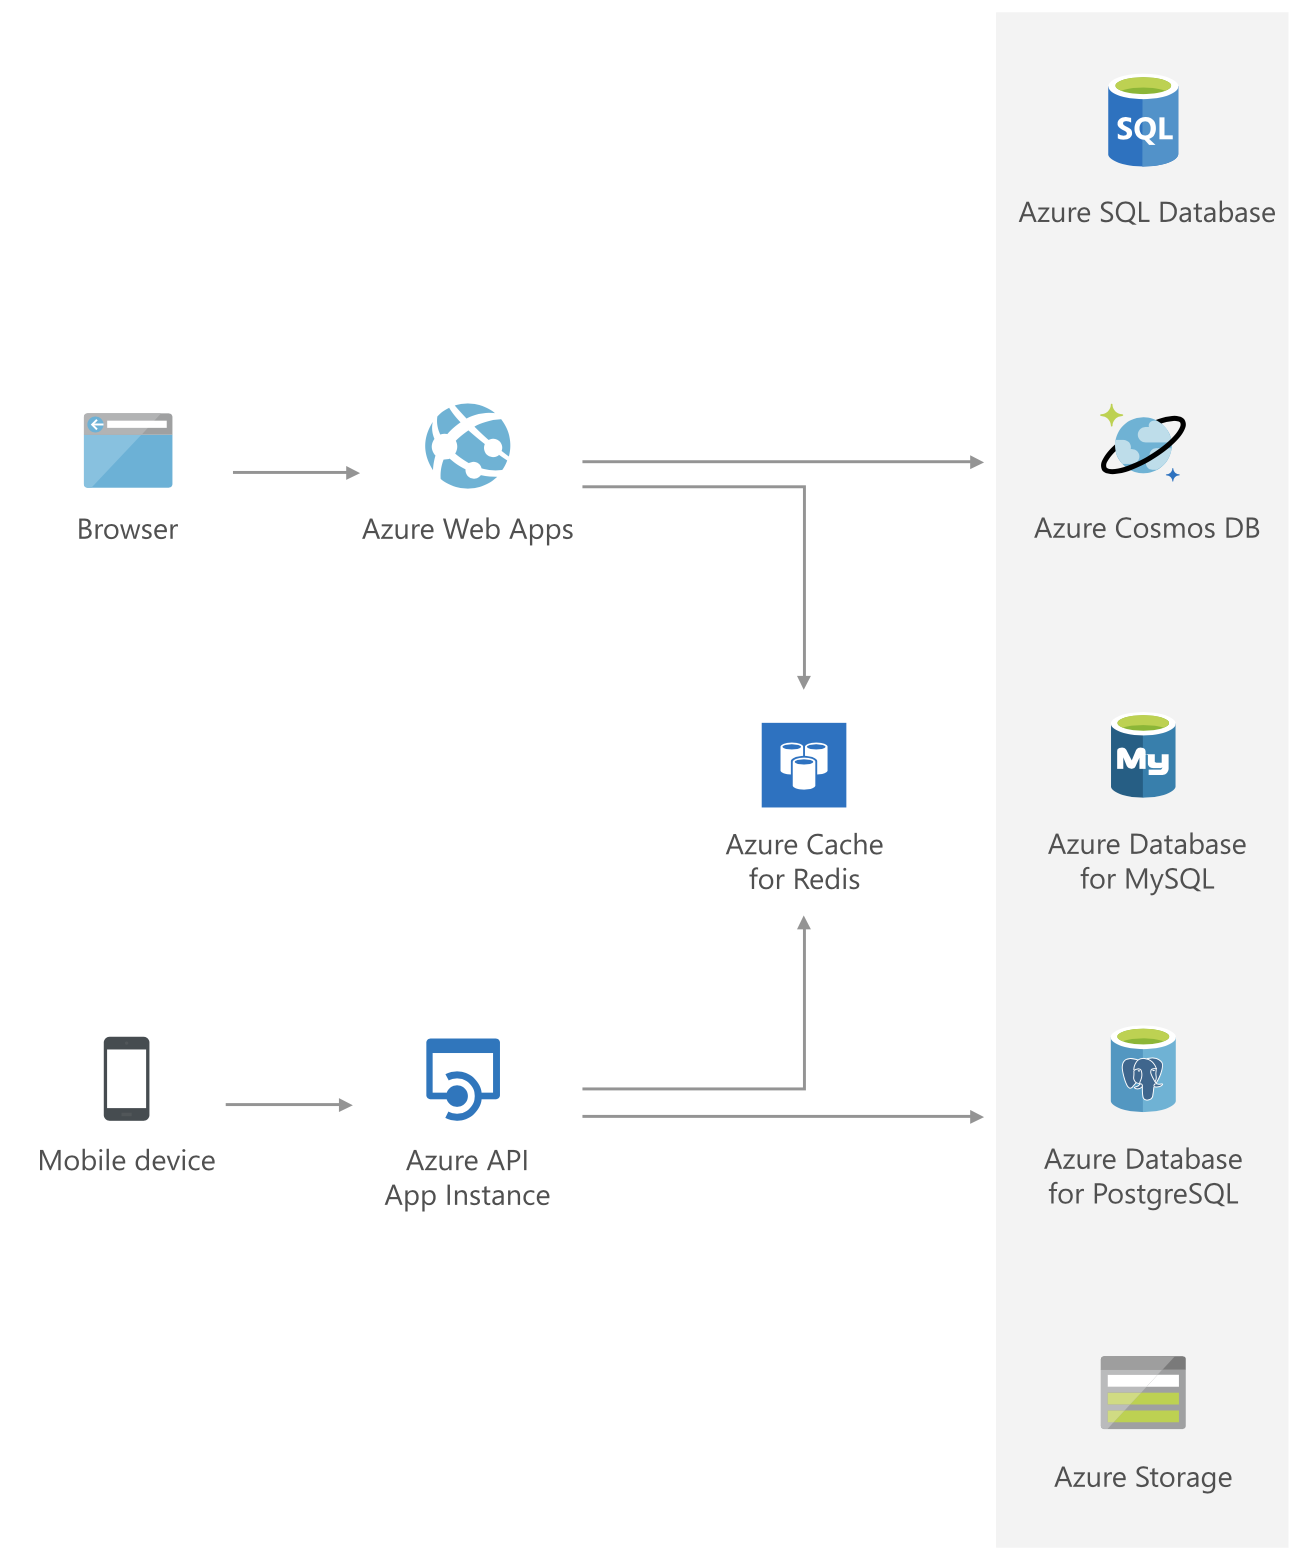
\includegraphics[width=0.5\linewidth]{cacheForRedis-integration}}%
	\caption{Azure Environment Integration}
\end{figure}

\subsection{Aerospike}
\label{ssec:aerospike}

Aerospike \cite{aerospike:1} is an enterprise-grade, high performance Key-Value Store. It is another \gls{KVS} technology currently available today. It promises a philosophy of \textit{"no data loss" } through Strong Consistency. Normal systems trade requiring this type of consistency usually trade performance for data integrity but Aerospike allows it  with minimal performance loss. That means it can be used for example in banking payments, retail and telecommunications use cases.

It also provides a dynamic cluster management and unique flexible storage. That enables very easy deployments and particularly very easy scalability, so it is able to meet any data volume needs and still maintaining low latencies across that wide range of data volumes, from low volumes until 100's \gls{TB} of data.

As for security, it includes (the enterprese version) a database access management and audit trail logs. It also includes transport level rncryption for client-server traffic and cross-datacenter traffic \cite{aerospike:2}.

\subsection{Discussion}
\label{ssec:s1_discussion}

In this chapter when gather information about the overview of th current Key-Value Store. We can conclude that the most important feature of this technology is the performance and all of the above products mentioned do focus on that characteristic. Some of them even compromise in another features to achieve the best performance possible. Security is not the main concern and the most used measures in the current technologies being securities implementations at the network and transport level by using \gls{TLS} and also full disk encryption. 

Network and transport layer security is a must when implementing any system, and this thesis will also use those standards. 

As for full disk encryption on the server, it opens up some attack vectors. Full disk encryption means that random users will not be able to query the data but credentialed users can. Although, anyone with full access to the database, for example database operators or/and administrators, can decrypt and access all information. This creates a risk of privacy breaking due to hackers wielding stolen credentials, rogue insiders who have been granted more access than they need or the well known honest-but-curious adversary model, where an administrator with full credentials does not have bad intentions, but, driven by curiosity, access information therefore breaking data privacy. A cloud based \gls{KVS} service like the ones talked above, this type of vulnerabilities can be a major concern for a use case with very sensitive data since the server would be off premises, there is no control over it when it comes to privacy of data.

This thesis will implemented a system based on Redis, the most popular and used Key-Value Store currently used and will try to solve some of the problems with security described above. It will compare the principle feature of a \gls{KVS}, the performance, of a simple and normal Redis server and a privacy-enhanced Redis solution so the user can calculate the trade-off between performance and security and applied the correspondent solution to their own use case.

\section{Trusted  Computing Environments} % (fold)
\label{sec:trusted_computing _environments}

In this section we will provide some additional considerations about some of the customizations available as class options.

\subsection{TPM – Trusted Platform Modules } % (fold)
\label{ssec:trusted_platform_modules}

The choice of the main language with the option “\texttt{lang=OPT}” affects:

\begin{itemize}
	\item \textbf{The order of the summaries.} First is printed the abstract in the main language and then in the foreign language. This means that if your main language for the document in English, you will see first the “abstract” (in English) and then the “resumo” (in Portuguese). If you switch the main language for the document for Portuguese, it will also automatically switch the order of the summaries to “resumo” and then “abstract”.
	\item \textbf{The names for document sectioning.} E.g., ``Chapter'' vs.\ ``Capítulo'', ``Table of Contents'' vs.\ ``Índice'', ``Figure'' vs.\ ``Figura'', etc.
	\item \textbf{The type of documents in the bibliogrpahy.} E.g., ``Technical Report'' vs.\ ``Relatório Técnico'', ``PhD Thesis'' vs.\ ``Tese de Doutoramento'', etc.
\end{itemize} 

No mater which language you chose, you will always have the appropriate hyphenation rules according to the language at that point. You always get Portuguese hyphenation rules in the ``Resumo'', english hyphenation rules in the ``Abstract'', and then the main language hyphenation rules for the rest of the document.

% subsection the_main_language (end).

% section additional_consideration (end)


\subsection{TPM - Enabled Software Attestation} % (fold)
\label{ssec:enabled _software_attestation}

You must choose the class of text for the document. The available options are:

\begin{enumerate}
	\item \textbf{bsc} --- BSc graduation report.
	\item \textbf{*mscplan} --- Preparation of MSc dissertation. This is a preliminary report graduate students at DI-FCT-NOVA must prepare to conclude the first semester of the two-semesters MSc work. The files specified by \verb!\dedicatoryfile! and \verb!\acknowledgmentsfile! are ignored, even if present, for this class of document.
	\item \textbf{msc} --- MSc dissertation.
	\item \textbf{phdprop} ---  Proposal for a PhD work. The files specified by \verb!\dedicatoryfile! and \verb!\acknowledgmentsfile! are ignored, even if present, for this class of document.
	\item \textbf{prepphd} ---  Preparation of a PhD thesis. This is a preliminary report PhD students at DI-FCT-NOVA must prepare before the end of the third semester of PhD work. The files specified by \verb!\dedicatoryfile! and \verb!\acknowledgmentsfile! are ignored, even if present, for this class of document.
	\item \textbf{phd} --- PhD dissertation.
\end{enumerate}
% subsection class_of_text (end)

% ============
% = Printing =
% ============
\subsection{HSM – Hardware Security Modules} % (fold)
\label{ssec:hardware_security_modules}

You must choose how your document will be printed. The available options are:
\begin{enumerate}
	\item \textbf{oneside} --- Single side page printing.
	\item \textbf{*twoside} --- Double sided page printing.
\end{enumerate}
% subsection printing (end)

% =============
% = Font Size =
% =============
\subsection{Trusted Execution Environments} % (fold)
\label{ssec:trusted_execution_environments}

You must select the encoding for your text. The available options are:
\begin{enumerate}
	\item \textbf{11pt} --- Eleven (11) points font size.
	\item \textbf{*12pt} --- Twelve (12) points font size. You should really stick to 12pt\ldots
\end{enumerate}
% subsection font_size (end)

% =================
% = Text encoding =
% =================
\subsection{Intel SGX} % (fold)
\label{ssec:Intel_sgx}

You must choose the font size for your document. The available options are:
\begin{enumerate}
	\item \textbf{latin1} --- Use Latin-1 (\href{http://en.wikipedia.org/wiki/ISO/IEC_8859-1}{ISO 8859-1}) encoding.  Most probably you should use this option if you use Windows;
	\item \textbf{utf8} --- Use \href{http://en.wikipedia.org/wiki/UTF-8}{UTF8} encoding.    Most probably you should use this option if you are not using Windows.
\end{enumerate}
% subsection font_size (end)

% ============
% = Examples =
% ============
\subsection{Sanctum} % (fold)
\label{ssec:sanctum}

Let's have a look at a couple of examples:

\begin{itemize}
	\item Preparation of PhD thesis, in portuguese, with 11pt size and to be printed single sided (I wonder why one would do this!)\\
	\verb!\documentclass[prepphd,pt,11pt,oneside,latin1]{thesisdifct-nova}!
	\item MSc dissertation, in english, with 12pt size and to be printed double sided\\
	\verb!\documentclass[msc,en,12pt,twoside,utf8]{thesisdifct-nova}!
\end{itemize}
% subsection examples (end)

\subsection{ARM Trust Zone} % fold
\label{ssec:arm_trust_zone}

ARM Trust Zone

\subsection{Discussion}
\label{ssec:s2_discussion}

Discussion

\section{TEE/SGX Enabled Key Value Stores} % (fold)
\label{sec:sgx_enabled_key_value_stores}

There has been an increase trend from developers to move their applications to the cloud. It provides dynamically and almost seamlessly scaling with predict cost. Although it also means that users need to rely on the cloud providers for securing and maintaining the integrity of their applications. That means the user must trust not only the provider's staff but also its globally distributed software and hardware not to expose their private data. Today's cloud providers only aim to protect their privileged code from the untrusted code (the user's code) and do not provide any guarantees about the opposite scenario.

To mitigate this use case, and after studying and discussing the Key-Value stores technologies and also the trusted platform modules as well as the trusted execution environments, in this chapter, it will be presented how are this two topics being combined and used together. 

It will be more focused on the Intel SGX platform as it is the one that will be used throughout this thesis. Currently, there are a number of databases who leverage this technology to provide a more secure environment and service. In the this chapter it's presented how they work and operate, discussed the differences between them and also the how the work planned to be performed on this thesis will solve some of the problems and caveats. 


\subsection{Trusted Execution with Intel SGX}
\label{ssec:trusted_execution_with_sgx}

As explained before, Intel SGX provides a trusted execution environment by running code inside the enclaves. It creates an isolated environment where we can run some instructions as securely as possible, without \gls{OS} intervention.

Key-Value Stores and other database type systems can leverage this secure and isolated environment to perform queries on very sensitive data that would otherwise be vulnerable to some attacks. There are a few techniques currently implemented to use isolated environments. Maintaining an encrypted database and using enclaves cryptographic capabilities to decrypt data and perform queries on plain text with the assurance of no data leaking is a possible use case. Also, maintaining a database fully on enclave memory, where it cannot be access by anyone other than the CPU is another way to keep the data secure by leveraging isolated and trusted execution environments. Different techniques will be furthermore discussed bellow. 

As we can see, isolated and trusted execution environments are an important feature when it comes to protecting the data from the \gls{OS} and Key-Values Store systems do benefit from them.

\subsection{Circumvention of SGX Limitations}
\label{ssec:circumvention_of_sgx_limitations}

There are a few limitations and challenges of the SGX platform that we address when programming for such technology.

It starts with a big challenge of choosing and defining what parts of the program can benefit of the \gls{SGX} security. As it is known, it works with two major application components, the trusted and untrusted modules of or program. The limitations have to be thoroughly analyzed so we can make that definition.  

The main limitations are: 

\begin{itemize}
	\item Performance
	\item Memory
	\item \gls{I/O}
	\item \gls{syscall}s
\end{itemize}

In the \gls{KVS} world, as we extensively covered, performance is the major concern and there is no real way around this limitation. Using secure enclaves will definitely decrease the supposed blazing fast performance. Although, with intelligent partition between the untrusted code, which will be fast, and the trusted instructions, which will be slower we can limit the performance overhead. By separating and well defining both modules of the application, we can decrease the code that needs to run securely and find a fine compromised between security and performance.

Memory sizing is also a limitation when using enclaves in \gls{SGX} technology. The amount of private secure data that can be maintained by the enclave is limited to the size of the enclave cache, which is around 128 \gls{MB}, being that only about 94 \gls{MB} are available to the application, with the rest reserved to metadata. Now, with \gls{SGX} v2 and for some operation systems, mainly Linux because of paging swap support, it can be increased up to all the memory available in the system \cite{sgx:1}. Although, page eviction to main untrusted memory introduces a big overhead because of encryption and decryption and integrity checks (2x - 2000x) \cite{scone:1}. Clever partitioning of the application into the untrusted and trusted modules will help to overcome this limitation as described in the next sections.

\gls{I/O} and \gls{syscall}s are limited by default on the enclave for security purposes, so it can't affect or be affected by the \gls{OS}. There is a way to perform and access \gls{I/O} and \gls{syscall}s through the aforementioned \gls{ECALL}s and \gls{OCALL}s (section \ref{ssec:Intel_sgx} of this thesis), but they have to be accounted for when implementing the application.

\subsection{SGX-Enabled Secure Databases}
\label{ssec:sgx_enabled_secure_databases}

Database management service developers are now implementing secure databases ready to take advantage of Intel \gls{SGX} hardware. It differs from normal databases because it runs on top of protected and encrypted memory so it can work with minimal \gls{TCB}.

Next subsections present and discuss the overview of the current technology that leverages \gls{SGX} to provide a secure database.

\subsubsection{EnclaveDB}
\label{sssec:enclave_db}

EnclaveDB \cite{enclavedb:1} is a privacy enhanced and secure database that works alongside with Intel \gls{SGX} and provides an Structured Query Language (SQL). It uses its technology to maintain all sensitive information inside \gls{SGX} enclaves in order to keep them secure from an threat model of strong adversaries that can control the entire software stack  on the database server. It resists attack from the administrator server, the database administrator and attacker who may compromised the operating system, the hypervisor or the database server.

Following Intel's application guidelines, EnclaveDB has an two part architecture: trusted (running on the enclave) and untrusted modules. The enclave hosts a query processing engine, natively compiled stored procedures and a trusted kernel which provides API's for sealing and remote attestation. The untrusted host process runs all other compo- nents of the database server. Figure \ref{fig:enclaveDB_architecture} shows the architecture of the enclaveDB server-side.

\begin{figure}[htbp]
	\centering
	{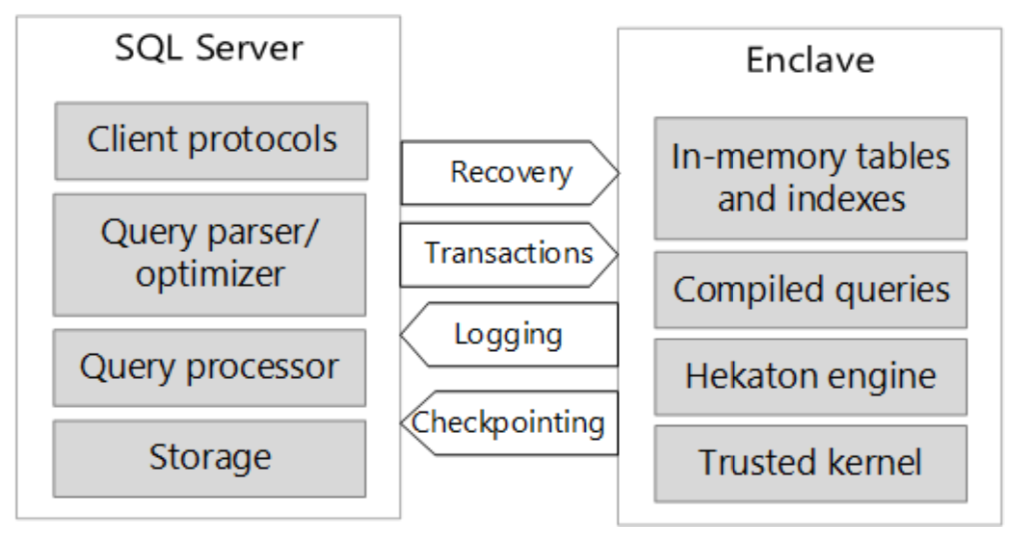
\includegraphics[width=0.5\linewidth]{enclaveDB_architecture}}%
	\caption{Server-side components of EnclaveDB}
	\label{fig:enclaveDB_architecture}
\end{figure}

Leveraging \gls{TEE}, EnclaveDB then provides a database with a \gls{SQL} interface and guarantees confidentiality and integrity with low overhead. With its design it also reduces the \gls{TCB} to a smaller set than any other "normal" database.

\subsubsection{Pesos DB}
\label{sssec:pesos_db}

Pesos \cite{pesos:1} is a secure implementation of object storage services like Amazon S3 \cite{s3:1}, Azure Blob Storage \cite{azureStorage:1}, Google Cloud Storage \cite{googleStorage:1} among others. In these current large-scale services, due to their complexity, the risk of confidentiality and integrity violations increase significantly. This storage systems are characterized by multiple layers of software and hardware stacked together which means the access policies for ensuring confidentiality and integrity are scattered across different code paths and configurations, thus exposing the data to more security vulnerabilities. Furthermore, untrusted third-party cloud platforms expose an additional risk of unauthorized data access by a malicious administrator.

Pesos allows clients to specify per-object security policies concisely and separately from the remaining storage stack. It also provides cryptographic attestation for the stored objects and their associated policies to verify the policy enforcement.

It enforces this policies by leveraging the Intel \gls{SGX} for trusted execution environments and Kinetic Object Storage \cite{kinetic:1} for trusted storage (secure storage - not the focus of this thesis). It structures a policy-compiler, its binary-format interpreter, per-object policy metadata, and the enforcement logic into a single layer of the storage stack. With this unification, it drastically reduces the \gls{TCB} when compared to the order cloud services. Then it uses the trusted execution environment provided by \gls{SGX} to connect directly Kinetic disk through an encrypted Ethernet connection allowing for object transfer and policy enforcement securely without any intermediate layers in the storage stack.

\subsubsection{Speicher}
\label{sssec:speicher}

Speicher \cite{speicher:1} is a secure \gls{LSM}-based Key-Value store that uses Intel \gls{SGX} and it ensures not only strong confidentiality and integrity properties, but also data freshness to protect against rollback/forking attacks. It leverages \gls{SGX} technology to achieve those security characteristics focusing on providing a \textbf{persistent} service, tolerant to system faults and securely recovering from crashes. It also tackles in interesting ways, two of the major limitations of \gls{SGX}: Memory Limits and Performance.

Implementing a Key-Value Store has a major requirement - High performance and low latency queries for big data structures. As already discussed, \gls{SGX} has some memory limits. The enclave memory is located in the Enclave Page Cache (\gls{EPC}) which is limited to 128 \gls{MB} with about 94 \gls{MB} available for application use (the rest being reserved for metadata). To allow creation of enclaves with bigger size than \gls{EPC}, the \gls{OS}  can use secure paging mechanism where it evicts pages to untrusted memory. Although with page encryption, decryption and integrity checks, this solution introduces high overheads (2× - 2000×) \cite{scone:1}.

To address this performance and memory problems, the developers of Speicher implemented the following custom features (from Speicher public paper):

\begin{itemize}
	\item \textit{"\textbf{I/O library for shielded execution}: Direct \gls{I/O} library for shielded execution. The \gls{I/O} library performs the \gls{I/O} operations without exiting the secure enclave; thus it avoids expensive system calls on the data path."}
	
	\item \textit{"\textbf{Asynchronous trusted monotonic counter}: Trusted counters to ensure data freshness. The counters leverage the lag in the sync operations in modern \gls{KVS} to asynchronously update the counters. Thus, they overcome the limitations of the native \gls{SGX} counters."}
	
	\item \textit{"\textbf{Secure \gls{LSM} data structure}: Secure \gls{LSM} data structure that resides outside of the enclave memory while ensuring the integrity, confidentiality and freshness of the data. Thus, the \gls{LSM} data structure overcomes the memory and \gls{I/O} limitations of Intel \gls{SGX}."}
\end{itemize}

The technology leverages \gls{SGX} with a clever partition between trusted and untrusted modules of the application. By maintaining the encrypted data on untrusted memory hardware it addresses the memory and persistent limitations, and by keeping some information in secure enclave memory and with a good \gls{I/O} library it overcomes (to an extent) the performance issues.

\subsubsection{ShieldStore}
\label{sssec:shieldstore}

ShieldStore \cite{shieldstore:1} is a \textit{"(...) shielded in-memory Key-Value Storage with \gls{SGX}"}. It aims to provide a very fast and low latency queries over very large data trying to overcome the \gls{SGX} memory limitation. It accomplice's it by maintaining the majority of the data structures in the non-enclave memory region, addressing as well the performance issue by not relaying on the page-oriented enclave memory extension provided by \gls{SGX}.

ShieldStore runs server-side in the enclave to protect encryption keys and for remote attestation and it is used to perform all the \gls{KVS} logic. It uses a hashed index structured but places it in the unprotected memory region instead of the enclave \gls{EPC}. As the main data structure is not protected by the \gls{SGX} hardware, each data entry must be encrypted by ShieldStore in the enclave, and written to the main hash table.

The main flow and architecture is as described on figure \ref{fig:shieldstore_overview}.

\begin{figure}[htbp]
	\centering
	{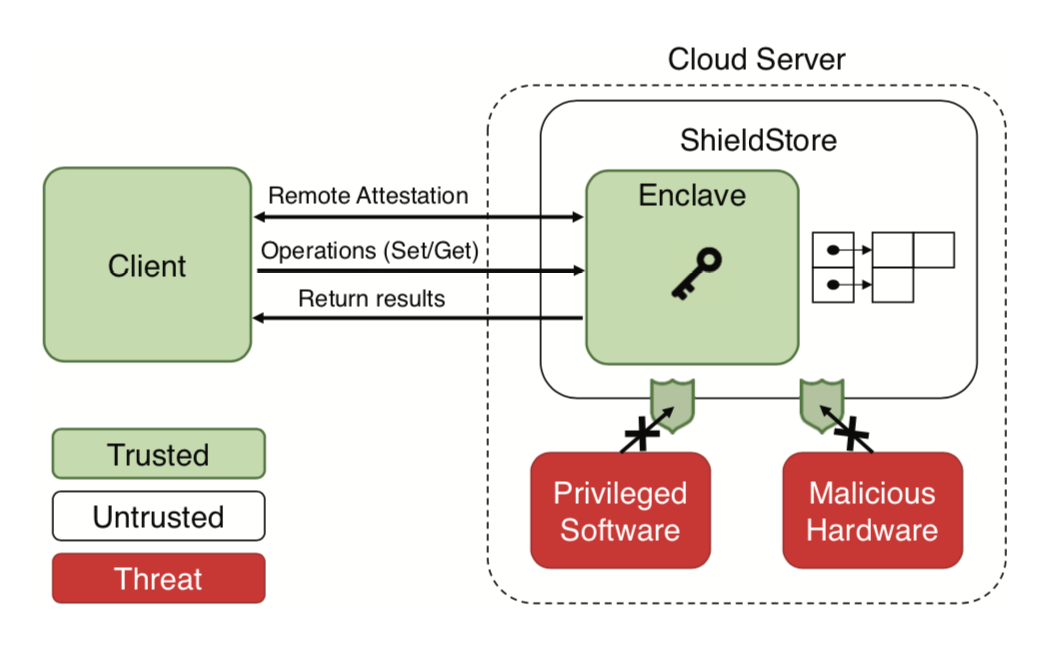
\includegraphics[width=0.5\linewidth]{shieldstore_flow}}%
	\caption{Overview of ShieldStore}
	\label{fig:shieldstore_overview}
\end{figure}

First the client remote attests the server-side (1) verifying \gls{SGX} support of the processor, the code, and other critical memory state of an enclave. In a second step, the client and the server exchange sessions keys (2) in order to establish a secure connection, using Intel \gls{SGX} libraries to do so. Using this newly generated session key, the client sends a request for an operation (3). The server deciphers and verifies the request and accesses the Key-Value Store (4). Clients do not access the server-side ciphertexts neither need to know the encryption key used by the server to encrypt the values. The server will then decrypt the data from the storage, encrypted it again with the session key and reply to the client (5). All accesses to the \gls{KVS} have integrity checks.

\subsection{Discussion}
\label{ssec:s3_discussion}

Discussion

% section how_to_write_using_latex (end)

\section{Related Work Balance and Critical Analysis}
\label{sec:related_work_balance_and_critical_analysis}
%
% \todo[inline]{A a note in a line by itself.}
%
Foo Bar
%
% Please note that
% \begin{center}
%   \textbf{\large this package and template are not official for FCT/NOVA}.
% \end{center}
